
%\setmonofont{Monaco}

\chapter{Desarrollo inicial del Sistema}

\newthought{En} Sistema Web que se desarrolló, se sistematizaron las siguientes
tareas:

\begin{itemize}
    \item El registro de los vehículos con las escaleras y el conductor.
    \item El registro de personas que ingresan a la empresa.
    \item El registro de mantenimiento a los vehículos.
    \item La emisión de reportes por vehículo, por parqueo, conductor y escaleras.
    \item Las notificaciones/alertas para el control del supervisor.
\end{itemize}

En este capítulo veremos como empleamos la metodología BDD en la fase inicial de
desarrollo del Sistema Web.

%\newthought{BDD}, como vimos plantea Escenarios para el desarrollo del sistema
%y luego se genera una código para hacer las pruebas usando la herramienta Behave.

\section{Escenarios del sistema}
Cada tarea a sistematizar llega a ser un comportamiento o funcionalidad para un
determinado usuario o rol.

\subsection{Registro de vehículos}
En este primer escenario nos interesa saber el día, la hora, el parqueo, el conductor
y las escaleras con las que sale y retorna.

Este primer {\it Feature} o {\it Característica} sera el {\it Registro de vehículos}
y lo guardaremos en el archivo {\it \bfseries registro.feature} con el siguiente contenido:

{\scriptsize
\begin{minted}{Gherkin}
Característica: Registro de vehículos
    Como un guardia
    Quiero registrar las salidas y retornos de los vehículos
    Para registrar los datos

    Esquema del escenario: Registrar vehículo de la empresa
        Dado que el vehículo con numero interno <interno>} esta de <estado>
        Y sale/retorna del parqueo <parqueo>
        Y con el conductor de con ítem <num_item>
        Y tiene el kilometraje <km>
        Y con las escaleras <escaleras>
        Y en fecha <fecha>
        Y en horas <hora>
        Cuando}} registre al vehículo <interno> con su estado de <estado>
        Y los datos del vehículo <interno> sean validos
        Entonces guardo el registro del vehículo <interno>
        Pero que pasa si el conductor del vehículo <interno> de retorno es diferente
        Y las escaleras del vehículo <interno> de retorno no son las mismas
        Y el parqueo de retorno del vehículo <interno> no es el mismo
        Y si el registro del vehículo <interno> tiene observaciones debe notificarse al supervisor
\end{minted}
}

Toda esta sintaxis ya vimos en el capitulo 3, pero ahora se presenta algo nuevo,
hay palabras que están dentro de {\bfseries $<$} y {\bfseries $>$}, esto también es
parte de la sintaxis de Gherkin, que es para el uso de tablas para los ejemplos.

{\scriptsize
\begin{minted}{Gherkin}
        Ejemplos: Datos de registro
            | parqueo  | interno | num_item | km    | escaleras | fecha      | hora  | estado  |
            | muyurina | 123     | 543      | 10100 | 23 43 12  | 18/02/2014 | 08:12 | salida  |
            | km 0     | 321     | 432      | 20100 | 45 14 54  | 18/02/2014 | 08:34 | salida  |
            | muyurina | I-02    | 564      | 15210 | 78 46 11  | 18/02/2014 | 08:43 | salida  |
            | muyurina | I-04    | 101      | 10010 | 99 98 90  | 18/02/2014 | 08:50 | salida  |
            | muyurina | I-01    | 110      | 12110 | 90 78 11  | 18/02/2014 | 08:58 | salida  |
            | muyurina | 321     | 432      | 20159 | 45 14     | 18/02/2014 | 10:05 | entrada |
            | muyurina | 321     | 432      | 20159 | 45 14 54  | 18/02/2014 | 10:50 | salida  |
            | taller   | 321     | 432      | 20249 | 45 14 54  | 18/02/2014 | 15:50 | entrada |
            | taller   | 321     | 432      | 20249 | 45 14 54  | 18/02/2014 | 18:10 | salida  |
            | muyurina | 123     | 505      | 10189 | 23 43 12  | 18/02/2014 | 18:52 | entrada |
            | muyurina | I-01    | 110      | 12184 | 90 78 11  | 18/02/2014 | 19:38 | entrada |
            | sucre    | I-02    | 564      | 15256 | 78 46 11  | 18/02/2014 | 20:00 | entrada |
            | muyurina | 321     | 432      | 20293 | 45 14 54  | 18/02/2014 | 20:35 | entrada |
            | muyurina | I-01    | 110      | 12184 | 90 78 11  | 19/02/2014 | 08:18 | salida  |
            | muyurina | I-04    | 1305     | 10000 | 99 98     | 19/02/2014 | 13:05 | entrada |
            | muyurina | I-01    | 120      | 12110 | 90 78 11  | 20/02/2014 | 08:58 | salida  |
            | muyurina | I-01    | 110      | 12987 | 90 78 11  | 25/02/2014 | 08:14 | entrada |
\end{minted}
}

En este comportamiento manejamos el rol de {\it Guardia} que llegaría a ser el Vigilante
Industrial, el se encarga de registrar a los vehículos de la empresa al sistema.
Este primer escenario es un caso ideal o como se dijo en el capítulo 3 es el
{\it camino feliz}, los siguientes escenarios muestran otras variables que manejan
los guardias al momento de registrar los vehículos ya sean de la empresa o no.

{\scriptsize
\begin{minted}{Gherkin}
Esquema del escenario: Registrar vehículo alquilado
    Dado que tiene la placa de control <placa>
    Y esta de <estado> del parqueo <parqueo>
    Y con el conductor con ítem <num_item>
    Y con las escaleras <escaleras>
    Y en fecha <fecha>
    Y en horas <hora>
    Cuando registre al vehículo con placa de control <placa>
    Y se validen los datos del vehículo alquilado
    Entonces registro el vehículo con placa de control <placa>

    Ejemplos: Datos de salida
        | parqueo  | placa    | num_item | escaleras | fecha      | hora  | estado  |
        | muyurina | 2341 GAB | 345      | 12 32 43  | 18/02/2014 | 08:00 | salida  |
        | km 0     | 212 BEN  | 456      | 44 55 76  | 18/02/2014 | 08:00 | salida  |
        | muyurina | 212 BEN  | 456      | 44 55 76  | 18/02/2014 | 11:10 | entrada |
        | muyurina | 212 BEN  | 456      | 44 55 76  | 18/02/2014 | 11:40 | salida  |
        | muyurina | 2341 GAB | 345      | 12 32 43  | 18/02/2014 | 18:05 | entrada |
        | km 0     | 212 BEN  | 456      | 44 55 76  | 18/02/2014 | 19:10 | entrada |
\end{minted}
}

{\scriptsize
\begin{minted}{Gherkin}
Esquema del escenario: Registrar vehículos que se quedan en parqueo
    Dado que que tiene el numero interno <num_interno>
    Y esta en el parqueo <parqueo>
    Y en fecha <fecha>
    Cuando registre el vehículo <num_interno>
    Entonces el vehículo se quedo en parqueo

    Ejemplos: Datos de vehículos que no salieron
        | parqueo  | num_interno | fecha     |
        | muyurina | I-02        | 8/05/2014 |

Esquema del escenario: Ingreso de vehículo externo
    Dado que ingresa una persona con documento <documento> a las oficinas <oficina>
    Y con numero de documento <num_doc>
    Y con el siguiente nombre <nombre>
    Y proviene de la ciudad <ciudad>
    Y con el siguiente motivo <motivo>
    Y con placa de vehículo <placa>
    Cuando registre a la persona <nombre> y el vehículo <placa>
    Y los datos sean validos
    Entonces registro a la persona <nombre> con el vehículo <placa>

    Ejemplos:
        | oficina  | documento | num_doc | nombre | ciudad | placa   | motivo               |
        | muyurina | pasaporte | 123456  | juan   | br     | 123 RRR | descarga de material |
        | central  | CI        | 654321  | carl   | lpz    | 321 GHF | descarga de material |
\end{minted}
}

Estos escenarios nos muestran las diferentes tareas que tienen que cumplir los
guardias, como registrar vehículos que no son de la empresa, vehículos alquilados
y vehículos de la empresa que no registran ninguna salida.

Para esta primera característica tendriamos un diagrama de secuencias de la
siguiente manera:

\begin{figure}[h]
  \begin{center}
    \def\svgwidth{\columnwidth}
    \input{figures/chapter4/sequence_register_car.pdf_tex}
%    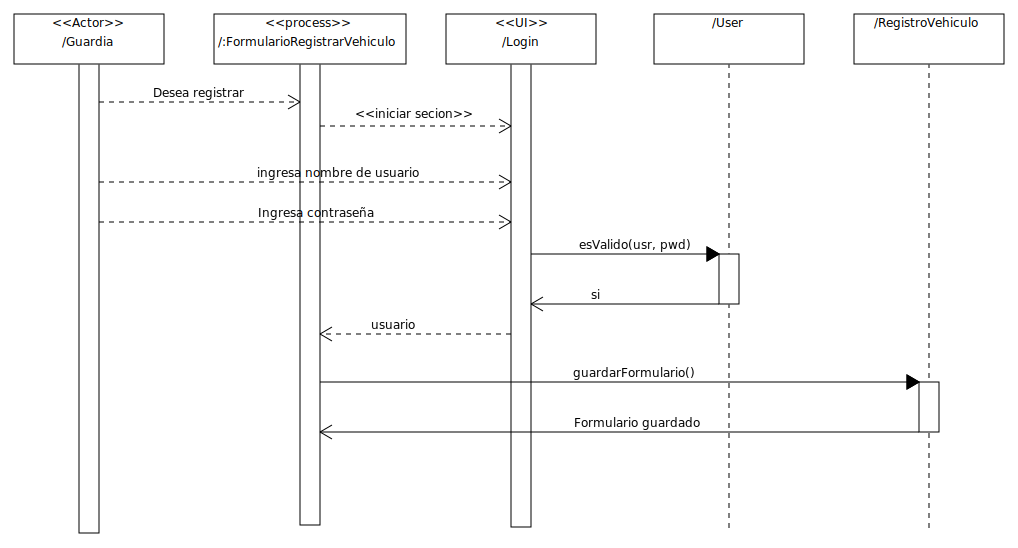
\includegraphics[width=1\textwidth]{figures/chapter4/SequenceDiagram21.svg}
    \caption[Diagrama de secuencia - Registro de vehículos]{
    Diagrama de secuencia para el Registro de vehículos}
  \end{center}
\end{figure}

\subsection{Registro de ingreso de personas}
Los guardias también tienen que estar atentos a toda {\it persona ajena} a la empresa
que quiere ingresar a las oficinas. Tiene que pedir un documento que lo identifique
y saber el motivo para lo que esta ingresando.

El archivo para este comportamiento sera {\it \bfseries ingresos.feature}

{\scriptsize
\begin{minted}{Gherkin}
Característica: Registro de personas
    Como un guardia
    Quiero registrar los ingresos y salidas de personas ajenas a la empresa
    Para tener un registro de ingresos

    Esquema del escenario: Registrar visita a oficinas
        Dado que ingresa una persona a las oficinas <oficina>
        Y con documento <documento>
        Y con numero de documento <num_doc>
        Y con el siguiente nombre <nombre>
        Y proviene de la ciudad <ciudad>
        Y con el siguiente motivo <motivo>
        Cuando registre a la persona
        Y el <num_doc> sea valido
        Entonces registro a la persona <nombre> con documento <num_doc> que ingreso a la oficina <oficina>

        Ejemplos:
            | oficina  | documento  | num_doc |   nombre     | ciudad |     motivo    |
            | muyurina | pasaporte  | 123456  | Marcelo Roca | br     | Reclamos ADSL |
            | central  | CI         | 654321  | Pedro Quispe | lpz    | Interac TV    |
\end{minted}
}

Para el registro de personas seguiría la siguiente secuencia.

\begin{figure}[h]
  \begin{center}
    \def\svgwidth{\columnwidth}
    \input{figures/chapter4/sequence_register_person.pdf_tex}
%    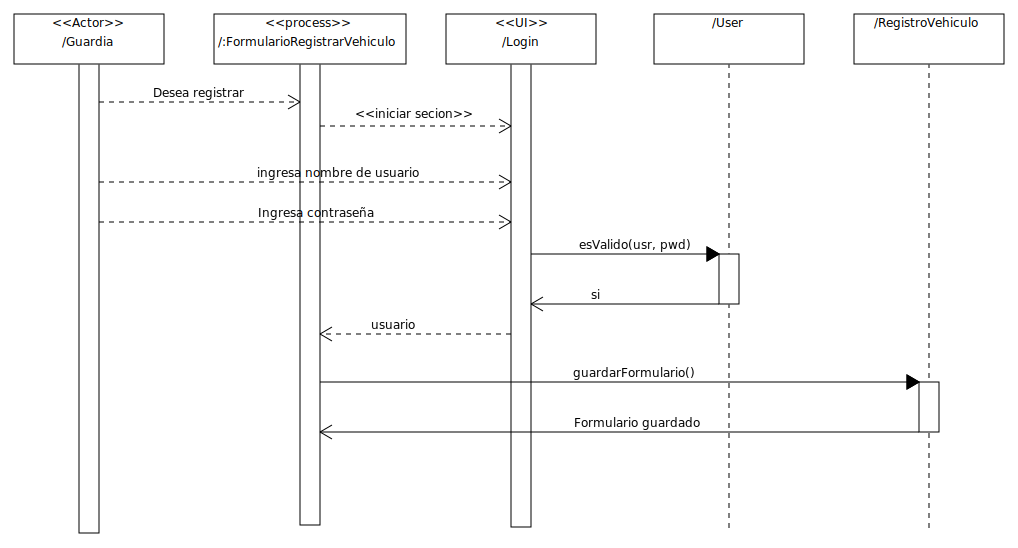
\includegraphics[width=1\textwidth]{figures/chapter4/SequenceDiagram21.svg}
    \caption[Diagrama de secuencia - Registro de personas]{
    Diagrama de secuencia para el Registro de Personas}
  \end{center}
\end{figure}

\subsection{Registro de mantenimiento}
Los vehículos siempre están en constante {\it mantenimiento},
pero también se vio la necesidad de tener un registro de que vehículos van al
taller para su mantenimiento y también programar mantenimientos preventivos.
Esta tarea la realiza el {\it Encargado de Vigilancia}.

El archivo para este comportamiento sera {\it \bfseries taller.feature}

{\scriptsize
\begin{minted}{Gherkin}
Característica: Registro de mantenimiento a vehículos
    Como un Encargado de Vigilancia
    Quiero registrar mantenimientos preventivos a los vehículos
    Para prevenir accidentes

    Esquema del escenario: Registrar o programar mantenimientos a vehículos
        Dado que el vehículo <interno> del parqueo <parqueo>
        Y su ultimo mantenimiento fue en fecha <fecha>
        Y con un kilometraje de <km_antiguo>
        Y con el siguiente motivo <motivo>
        Y su kilometraje actual es <km_actual>
        Y requiere el siguiente mantenimiento <mantenimiento>
        Cuando registre a el mantenimiento
        Y los datos de registro sean validos
        Entonces registro al vehículo <interno> del parqueo <parqueo> para mantenimiento

        Ejemplos:
            | parqueo  | interno | fecha       | km_antiguo | motivo           | km_actual | mantenimiento     |
            | muyurina | 167     | 12/01/2014  | 167944     | cambio de aceite | 187983    | cambio de aceite   |
            | sucre    | 54      | 25/04/2014  | 110456     | chequeo de motor | 150876    | revisión de motor |
\end{minted}
}

El diagrama de secuencia seria el siguiente:

\begin{figure}[h]
  \begin{center}
    \def\svgscale{0.6}
    \input{figures/chapter4/sequence_register_maintenance.pdf_tex}
%    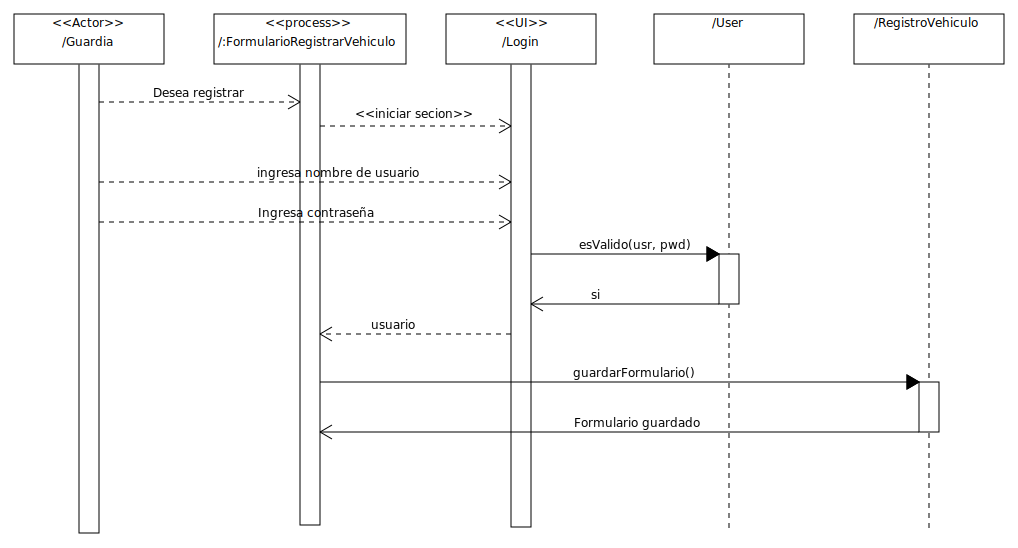
\includegraphics[width=1\textwidth]{figures/chapter4/SequenceDiagram21.svg}
    \caption[Diagrama de secuencia - Programar mantenimiento]{
    Diagrama de secuencia para programar mantenimiento}
  \end{center}
\end{figure}
\subsection{Reportes}
Los {\it reportes} es algo fundamental en el Sistema Web que se desarrolló, porque ayuda
a hacer los diferentes seguimientos de cada parqueo de los vehículos de la empresa.
Esta es una tarea que solo lo puede hacer el {\it Encargado de Vigilancia}.

El archivo para este comportamiento sera {\it \bfseries reportes.feature}

{\scriptsize
\begin{minted}{Gherkin}
Característica: Pagina de reportes
    Como un Encargado de Vigilancia
    Quiero sacar reportes de vehículos
    Para control interno

    Esquema del escenario: Sacar reportes de parqueos de un día
        Dado que necesito el reporte del parqueo <parqueo>
        Y solo de la fecha <fecha>
        Y lo quiero en formato <formato>
        Cuando ingreso los datos
        Entonces saco el reporte

        Ejemplos:
            | parqueo  | fecha       | formato |
            | muyurina | 10/06/2014  | pdf     |
            | sucre    | 15/07/2014  | excel   |

    Esquema del escenario: Sacar reportes de parqueos de un rango de fechas
        Dado que necesito el reporte del parqueo <parqueo>
        Y con fecha inicial <fecha_inicial>
        Y con fecha final <fecha_final>
        Y lo quiero en formato <formato>
        Cuando ingreso los datos
        Entonces saco el reporte

        Ejemplos:
            | parqueo  | fecha_inicial | fecha_final | formato |
            | muyurina | 10/03/2014    | 26/06/2014  | pdf     |
            | sucre    | 15/07/2014    | 26/06/2014  | excel   |
\end{minted}
}

La gran ventaja que tiene hacer estos escenarios en un lenguaje que entiende el
cliente es que puede dar su opinión de acuerdo a que variables quiere que también
se contemplen. Por ejemplo, en los anteriores escenarios para los reportes el
cliente vio la necesidad de tener también reportes que filtren por ítem de conductor
y por el número interno del vehículo. Dado estas aclaraciones con el cliente
el escenario quedaría de la siguiente manera:

{\scriptsize
\begin{minted}{Gherkin}
Esquema del escenario: Sacar reportes de parqueos
    Dado que necesito el reporte del parqueo <parqueo>
    Y con fecha inicial <fecha_inicial>
    Y con fecha final <fecha_final>
    Y con conductor <item_conductor>
    Y del vehículo <interno>
    Y lo quiero en formato <formato>
    Cuando ingreso los datos
    Entonces saco el reporte

    Ejemplos:
        | parqueo  | fecha_inicial | fecha_final | item_conductor | interno | formato |
        | muyurina | 10/03/2014    | 26/06/2014  | 505            | 167     | pdf     |
        | sucre    | 15/07/2014    | 26/06/2014  | 543            | I-02    | excel   |
\end{minted}
}

\begin{figure}[h]
  \begin{center}
    \def\svgwidth{\columnwidth}
    \input{figures/chapter4/sequence_report.pdf_tex}
%    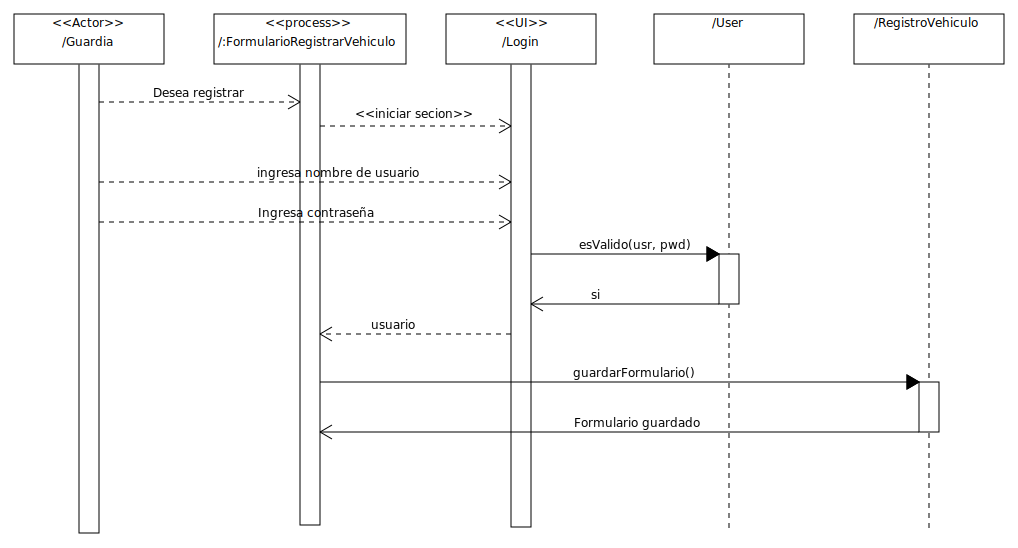
\includegraphics[width=1\textwidth]{figures/chapter4/SequenceDiagram21.svg}
    \caption[Diagrama de secuencia - Solicitud de reportes]{
    Diagrama de secuencia para la emisión de reportes}
  \end{center}
\end{figure}

\subsection{Notificaciones}
Las {\it notificaciones} ayuda al {\it Encargado de Vigilancia} a tomar ciertas medidas
de seguridad en la empresa, mas que todo respecto a los vehículos de la empresa y
los conductores.

Las notificaciones que se manejan están medidos por {\it bajo, medio y alto} solo
para estas alertas:

\begin{itemize}
  \item Un vehículo se queda en un parqueo diferente al que esta asignado - {\it medio}
  \item Un vehículo no llega a ningún parqueo - {\it alto}
  \item La licencia de conducir de un conductor ya esta por vencer - {\it alto}
\end{itemize}

El archivo para este comportamiento sera {\it \bfseries notificaciones.feature}

{\scriptsize
\begin{minted}{Gherkin}
Característica: Personalizar notificaciones
    Como un Encargado de Vigilancia
    Quiero dar valor a las notificaciones
    Para tomar medidas de seguridad

    Esquema del escenario: Cargar notificaciones
        Dado que manejo varias notificaciones
        Y con valores diferentes
        Cuando asigno valor a las notificaciones
        Entonces el sistema debe mandar alertas al encargado
\end{minted}
}

El diagrama de secuencia seria el siguiente:

\begin{figure}[h]
  \begin{center}
    \def\svgwidth{\columnwidth}
    \input{figures/chapter4/sequence_notifications.pdf_tex}
    \caption[Diagrama de secuencia - Administrar notificaciones]{
    Diagrama de secuencia para la administración de notificaciones}
  \end{center}
\end{figure}

Hasta este punto tenemos claro que es lo que tiene que hacer el sistema, que funcionalidades
debe cumplir, lo que veremos a continuación es como podemos darle un valor agregado
a todo los escenarios que escribimos con la ayuda de {\it Behave}

\section{Código generado para los test}
{\it Behave} es un interprete de Gherkin que lee todas las especificaciones que
escribimos y la forma de ejecutarlo es de la siguiente manera\footnote{En el Anexo A
se mostrará como instalar y configurar las diferentes herramientas}:

\vspace{0.5cm}
\texttt{\$ {\bfseries behave} \emph{registro.feature}}
\vspace{0.5cm}

\begin{figure}[h]
  \begin{center}
  \includegraphics[width=0.8\textwidth]{figures/chapter4/behave01m.png}
  \caption[Behave - primera ejecución]{Ejecución de behave}
\end{center}
\end{figure}

Todas las letras que nos muestra en color naranja son \emph{pasos} o \emph{steps}
sin definir y lo que nos muestra es un ejemplo de como podemos escribir estos
pasos. En el Anexo B de los \emph{Test de Ejecución} encontrará este código.

Los archivos \emph{.feature} tienen que estar en un directorio llamado {\bfseries
features} y el código escrito en python tiene que estar en otro directorio
llamado {\bfseries steps}, como puede ver a continuación.

\begin{figure}[h]
  \begin{center}
  \includegraphics[width=0.9\textwidth]{figures/chapter4/features_dir.png}
  \caption[Directorio features]{Organización del directorio \emph{features}}
\end{center}
\end{figure}

Esta es la forma correcta de organizar los features y los steps para Behave,
ademas en este directorio encontramos dos archivos nuevos que son:

\vspace{0.5cm}
\begin{mdframed}
\noindent
\texttt{
behave.ini \\
environment.py
}
\end{mdframed}
\vspace{0.5cm}

En {\bfseries behave.ini} escribimos variables de entorno que usara Behave al
momento de interpretar los archivos {\it .features}

\begin{verbatim}
[behave]
lang = es
\end{verbatim}

En este caso solo definimos el lenguaje en el que están escritos los escenarios.

En {\bfseries environment.py} inicializamos variables que usaremos al momento de
ejecutar los test.

\begin{verbatim}
import logging

def before_all(context):
    context.register_car = None
    context.parqueo_out = None
    context.km_out = None
    context.escaleras_out = None
    context.item_out = None
    context.date_out = None
    context.time_out = None
    context.dict_cars = {}
    context.warning = False

    if not context.config.log_capture:
        logging.basicConfig(level=logging.DEBUG)
\end{verbatim}

En los test que ejecutamos para este proyecto necesitamos que estén inicializadas
todas estas variables antes de todo.

Veamos como ejemplo la ejecución del {\it{\bfseries registro.feature}}:

\texttt{\$ {\bfseries behave} \emph{registro.feature}}

\begin{figure}[h]
  \begin{center}
  \includegraphics[width=1.1\textwidth]{figures/chapter4/behave_registro.png}
  \caption[Ejecución con Behave con error]{Ejecución con Behave escenario con error}
\end{center}
\end{figure}

En esta parte de la ejecución los colores nos interesan:

\begin{itemize}
  \item Verde. Se ejecuta el paso o {\it step} sin errores.
    \item Rojo. Ocurrió un error al ejecutar el paso.
    \item Azul. Pasos que no se ejecutaron.
    \item Naranja. Pasos no definidos.
\end{itemize}

En el escenario anterior hay un error, pero mas que un error es una alerta o futura
notificación en el sistema, ya que el vehículo ingresa al parqueo pero la persona
que ingresa con el vehículo no es la misma que lo saco. El sistema debe ser capaz
de agarrar esa alerta al momento de registrar y crear una notificación para el
encargado de Vigilancia.

En el siguiente escenario se ejecuta cada paso sin error:

\begin{figure}[h]
  \begin{center}
  \includegraphics[width=1.1\textwidth]{figures/chapter4/behave_registro02.png}
  \caption[Ejecución con Behave sin error]{Ejecución con Behave, escenario sin error}
\end{center}
\end{figure}

En esta fase inicial del desarrollo del producto tenemos claro de todas las
funcionalidades que espera ver el cliente en el sistema. Con todo lo desarrollado
hasta el momento y los test escritos en {\it Behave} se tiene como un primer
producto entregable, donde mostramos al cliente como pasan los test de acuerdo a
las especificaciones.

A continuación veremos como se hizo el modelo de la Base de Datos teniendo en
mente todo lo que hicimos hasta este punto. Hablando en términos de BDD hasta este
punto del desarrollo es trabajo de los testers y desarrolladores, de aquí para
adelante es solo trabajo de los desarrolladores.

\section{Modelo del sistema}
Según la definición original de BDD expuesta por Dan North\footnote{Dan North,
  principal impulsor en el desarrollo de BDD, \url{http://dantnorth.net}
consultado el 7/07/2014} nos dice:
\vspace{0.5cm}
\begin{mdframed}
{\it BDD is a second-generation, outside–in, pull-based, multiple-stakeholder,
  multiple-scale,  high-automation, agile methodology. It describes a cycle of
  interactions with well-defined outputs, resulting in the delivery of working,
  tested software that matters.
}
\end{mdframed}
\vspace{0.5cm}
BDD es pensar de afuera hacia adentro({\it outside-in}), es decir, una vez que
ya tenemos bien pensadas y trabajadas las funcionalidades, eso nos ayuda a tener una
idea más clara de lo que tenemos que hacer, como ser los modelos a implementar y
los roles que son necesarios crear.

\subsection{ACL - Lista de Control de Acceso}
Según las características podemos identificar dos roles: {\it Encargado de Vigilancia}
y {\it Guardia}, que son los que trabajaran con el sistema. Con ACL podemos definir
que puede y que no puede hacer cada rol, como vemos a continuación.

\vspace{1.0cm}

\begin{figure}[h]
  \begin{center}
  \includegraphics[width=0.7\textwidth]{figures/chapter4/acl.png}
  \caption[ACL - Roles del sistema]{ACL - Lista de Control de Acceso}
\end{center}
\end{figure}

\vspace{0.5cm}

En la figura anterior se muestra en las columnas las acciones sobre
un recurso y en las filas se tiene a los roles definidos en el sistema, en cada
intersección existe un valor de {\it falso} o {\it verdadero} que indica si el
rol tiene permiso de realizar esta acción o si no la tiene.

Esto es de acuerdo a las acciones que realizaran en el sistema:

\begin{itemize}
  \item como {\it guardia} debe ser capaz de registrar a los vehículos, es decir
    crear nuevos registros.
  \item como {\it guardia} debe ser capaz de ver todos los registros guardados.
  \item como {\it guardia} debe ser capaz de ver los reportes.
  \item como {\it encargado de vigilancia} debe ser capaz de editar registros.
  \item como {\it encargado de vigilancia} debe ser capaz de borrar registros.
  \item como {\it encargado de vigilancia} debe ser capaz de crear usuarios.
\end{itemize}

Este enfoque fue el más flexible que se encontró y es el que se implemento en la
aplicación.

Guiándonos por los escenarios que vimos en la sección 4.1 nosotros podemos ir
modelando con una idea mas clara de que actores o entidades necesitaremos para
cada característica.

\subsection{Registro de vehículos}
En base a nuestra primera característica que es el registro de vehículos y los
escenarios que la componen tendremos las siguientes entidades para un modelo ER.

%\begin{figure}[h]
%  \begin{center}
%    \def\svgwidth{\columnwidth}
%    \input{figures/chapter4/sequence_reg_car.pdf_tex}
%%    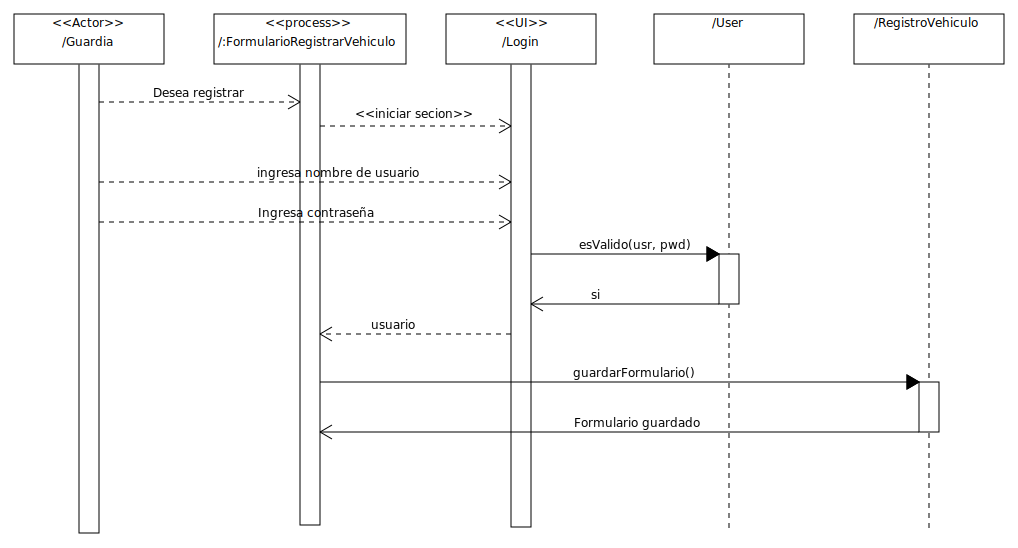
\includegraphics[width=1\textwidth]{figures/chapter4/SequenceDiagram21.svg}
%    \caption[Diagrama de casos de uso - Registro de vehículos]{
%    Diagrama de casos de uso para el Registro de vehículos}
%  \end{center}
%\end{figure}

\begin{itemize}
    \item User. Representa al usuario que usa el sistema, para este escenario el
      usuario es directamente el {\it guardia}.
    \item Employee. Es el empleado o funcionario que sale o retorna con el vehículo.
    \item BranchOffice. La sucursal de donde sale o ingresa el vehículo.
    \item Car. El Vehículo que es registrado.
    \item CarRegistration. La tabla donde se registra todos las salidas y retornos
        de los vehículos.
\end{itemize}

\begin{figure}[h]
  \begin{center}
    \includegraphics[width=0.6\textwidth]{figures/chapter4/er_registro.png}
    \caption[Modelo ER - Registro de vehículos]{Modelo ER para el registro de vehículos}
  \end{center}
\end{figure}

\newpage
\subsection{Registrar ingresos a oficinas}
En base al escenario de {\it ingreso de personas a la empresa} tenemos las
siguientes entidades con su modelo ER respectivo:

\begin{itemize}
    \item User. Representa al usuario que usa el sistema, para este escenario el
      usuario es directamente el {\it guardia}.
    \item Guest. Es la persona que esta ingresando a la empresa.
    \item RegisterGuest. La tabla donde se registran todos los ingresos.
\end{itemize}

\begin{figure}[h]
  \begin{center}
    \includegraphics[width=0.5\textwidth]{figures/chapter4/er_reg_visitas.png}
    \caption[Modelo ER - Registro de visitas]{Modelo ER para el registro de visitas}
  \end{center}
\end{figure}

\subsection{Programar mantenimiento}
Para programar mantenimiento de los vehículos se requieren las siguientes
entidades:

\begin{itemize}
    \item Car. El vehículo que es registrado.
    \item BranchOffice. La sucursal a la que pertenece el vehículo.
    \item MaintenanceProgram. La tabla donde se registra el mantenimiento programado.
\end{itemize}

\begin{figure}[h]
  \begin{center}
    \includegraphics[width=0.6\textwidth]{figures/chapter4/er_prog_mant.png}
    \caption[Modelo ER - Programar mantenimiento]{Modelo ER para programar mantenimiento}
  \end{center}
\end{figure}

\subsection{Registrar salida a taller}
Las entidades que están involucradas son las mismas que las de registro de ingreso
y salida de vehículos excepto que en este escenario tenemos una entidad más, que
es la entidad {\it MaintenanceWorkshop} o taller que es donde se registra cada
ingreso de un vehículo al taller de la empresa para su reparación o mantenimiento.

\begin{itemize}
    \item User. Representa al usuario que usa el sistema, para este escenario el
      usuario es directamente el {\it guardia}.
    \item Employee. Es el empleado o funcionario que sale o retorna con el vehículo.
    \item BranchOffice. La sucursal de donde sale o ingresa el vehículo.
    \item Car. El Vehículo que es registrado.
    \item CarRegistration. La tabla donde se registra todos las salidas y retornos
        de los vehículos.
    \item MaintenanceWorkshop. Tabla donde se registra el ingreso de los vehículos al
      taller de la empresa para su mantenimiento o reparación.
\end{itemize}

\begin{figure}[h]
  \begin{center}
    \includegraphics[width=0.8\textwidth]{figures/chapter4/er_salida_taller.png}
    \caption[Modelo ER - Registro de salida a taller]{Modelo ER para el registro de salida a taller}
  \end{center}
\end{figure}

\subsection{Administrar notificaciones}
Las notificaciones tienen la lógica de quien envía {\it sender} o la crea y para
quien es la notificación {\it owner}.

\begin{itemize}
    \item User. El usuario que envía la notificación o al que le corresponde.
    \item Notifications. Las notificaciones con sus respectivos dueños y con la
      prioridad que le corresponde.
    \item Notification. Las notificaciones creadas.
\end{itemize}

\begin{figure}[h]
  \begin{center}
    \includegraphics[width=0.8\textwidth]{figures/chapter4/er_notificaciones.png}
    \caption[Modelo ER - Notificaciones]{Modelo ER para el manejo de notificaciones}
  \end{center}
\end{figure}

\newpage
Aqui terminamos este desarrollo inicial del sistema, con los siguientes logros:

\begin{itemize}
    \item Funcionalidades escritas con BDD y probadas con Behave, mostrando así
      como se ejecuta cada funcionalidad.
    \item Modelo ER de la Base de Datos
\end{itemize}

En el siguiente capítulo veremos la parte del desarrollo web y el uso del
framework Django.

%En esta fase inicial del desarrollo del producto tenemos claro de todas las
%funcionalidades que espera ver el cliente en el sistema. Con todo lo desarrollado
%hasta el momento y los test escritos en {\it behave} se tiene como un primer
%producto entregable, donde mostramos al cliente como pasan los test de acuerdo a
%las especificaciones.

%En el libro \cite{Eigen1971} y en el libro \bibentry{Knuth1968} y usando el libro
%de latex \cite{goossens93}

